\documentclass[draft,onefignum,onetabnum]{siamart190516}

\usepackage{lipsum}
\usepackage{amsfonts}
\usepackage{graphicx}
\usepackage{epstopdf}
\usepackage{tikz}
\usepackage[caption=false]{subfig}
\usepackage{algorithmic}
\ifpdf
  \DeclareGraphicsExtensions{.eps,.pdf,.png,.jpg}
\else
  \DeclareGraphicsExtensions{.eps}
\fi

\headers{Infinite domain Helmholtz equation}{Anil Zengino\u{g}lu}


\usepackage{mathrsfs}
\usepackage{mathtools}
%\usepackage{wasysym}
%\usepackage{amssymb}
%\usepackage{amsmath}

\DeclareSymbolFontAlphabet{\mathrsfs}{rsfs}
\newcommand{\scri}{\mathrsfs{I}}

\newcommand{\be}{\begin{equation}}
\newcommand{\ee}{\end{equation}}
\newcommand{\iu}{{i\mkern1mu}}
%\newcommand{\iu}{\mathrm{i}}
\DeclareMathOperator\arctanh{arctanh}


\title{A null infinity layer for wave scattering}

\author{Anil Zengino\u{g}lu\thanks{Institute for Physical Science and Technology, University of Maryland, College Park, MD 20742
  (\email{anil@umd.edu)}.}}

\usepackage{amsopn}

\date{}


\begin{document}

\maketitle

\begin{abstract}
We solve time-harmonic wave scattering problems on unbounded domains. The technique, first developed in numerical relativity for time-domain wave equations, maps the unbounded domain to a bounded domain and scales out the known oscillatory decay towards infinity. We design a layer for the infinite exterior domain that restricts the transformations to an annular domain. The method does not require the local Green function and can therefore be applied to a wide range of problems including variable coefficients and nonlinear source terms. The method's main advantages are the exact treatment of the local boundary and access to radiative fields at infinity. The freedom in the transformations allows us to choose parameters adapted to high-frequency wave propagation in the exterior domain. We demonstrate the technique's efficiency in one- and two-dimensional numerical examples.
\end{abstract}

\begin{keywords}
	Helmholtz equation, unbounded domain, high wavenumbers, null infinity %,hyperboloidal 
\end{keywords}

\begin{AMS}
	65N35, %(Spectral,  collocation  and  related  methods  forboundary value problems involving PDEs)
	65H05, %(Numerical  computation  of  solutions  to  singleequations)
	65N22, %(Numerical  solution  of  discretized  equations  forboundary value problems involving PDEs)
	65N06, %(Finite  difference  methods  for  boundary  valueproblems involving PDEs)
	65F05, %(Direct numerical methods for linear systems and matrix inversion)
	35J05  % (Laplace  operator,  Helmholtz  equation)
\end{AMS}


%%%%%%%%%%%%%%%%%%%%%%%%%%%%%%
\section{Introduction}
%%%%%%%%%%%%%%%%%%%%%%%%%%%%%%

% General background of the problem
%%%%%%%%%%%%%%%%%%%%%%%%%%%%%%
\subsection{The problem}
Wave propagation problems on unbounded domains appear in many areas of science and technology. The equations that describe these problems vary widely in complexity and structure: scalar wave equations describe acoustic and seismic waves, vector wave equations describe electromagnetic waves, and tensor wave equations describe gravitational waves. The equations may have variable coefficients or include nonlinear terms depending on the application. Despite this diversity, solutions to wave equations share some essential properties.

Generally, wave equations have oscillatory solutions that propagate to infinity. While the meaning of oscillatory solutions is intuitively clear, propagation to infinity is harder to understand. What is meant by this statement is that generic solutions to wave equations decay slowly. When the energy of a propagating wave is conserved, the amplitude of the wave in $d$-dimensional space decays only as $r^{\frac{1-d}{2}}$ where $r$ denotes the distance to the source of the wave. 

This slow decay is what makes waves important in applications because we can measure them far away from the source. The computation of the far-field pattern is the primary goal in many problems. The echo area for acoustic waves, the radar cross section for electromagnetic scattering, or the gravitational flux are all defined with a limit to infinite distance. The relevance of the behavior of solutions at infinity makes numerical calculations of wave equations a difficult problem.

The task is to compute oscillatory solutions on infinite domains. Consider a time-harmonic plane wave that fills out the entire spatial domain, $e^{\iu k r}$, with wavenumber $k$ on $r\in[0,\infty)$. \emph{How can we solve an equation describing infinitely many oscillations with the finite resources of a computer?}

This paper answers the above question by employing relativistic methods, in particular, the unification of space and time into spacetime, conformal structure, and hyperbolic geometry. They allow us to compute oscillatory solutions to time-harmonic wave equations on unbounded domains without resorting to approximations other than numerical discretization. The methods are agnostic of the fundamental solution, and can therefore be applied to a wide variety of problems in science and engineering.

% Problem description and past effort
%%%%%%%%%%%%%%%%%%%%%%%%%%%%%%
\subsection{Helmholtz equation}
One of the simplest cases where the computational difficulties with wave equations are apparent is the linear, constant-coefficient, source-free Helmholtz equation. Consider the problem of time-harmonic wave scattering from a bounded obstacle $D \subset \mathbb{R}^d$ in $d$ dimensions. The scattered wave, $U$, satisfies the Helmholtz equation and the Sommerfeld radiation condition at infinity
\begin{equation}
	\label{eq:helm}
	\begin{gathered}
		\Delta U + k^2 U = F \quad \mathrm{in } \ \mathbb{R}^d\setminus \bar{D}, \\
		\partial_r U - \iu k U = o\left(r^{\frac{1-d}{2}}\right) \quad \mathrm{as} \ r\to\infty,\ d=1,2,3.
	\end{gathered}
\end{equation}
Dirichlet or Neumann conditions are given on the surface of the scatterer $D$. The two computational difficulties for this problem are: (i) the unbounded domain and (ii) the highly oscillatory behavior of the solution for high wavenumbers $k$. Both difficulties have been active areas of research with an extensive list of proposed treatments (see reviews \cite{TSYNKOV1998465, HagstromReview, engquist2003computational}).

% Past effort
Methods for handling the unbounded domain fall into two main categories: local and exact \cite{TSYNKOV1998465, HagstromReview, givoli2013numerical}. The term exact refers boundary treatments that are free from approximations other than discretization. Local methods are convenient but approximate, while exact methods are accurate but cumbersome. 

Local methods are most common due to their convenience and generality. They include high-order boundary conditions \cite{EngquistMajda77, BaylissTurkel80} and absorbing regions \cite{israeli1981approximation, BERENGER1994185}. A prominent example of absorbing regions is the perfectly matched layer \cite{BERENGER1994185} where solutions to wave equations are damped exponentially thereby avoiding reflections from the outer boundary. Among high-order boundary conditions, there are spectrally convergent local methods that may be sufficiently accurate for many applications \cite{hagstrom2009complete}. 

Exact methods, on the other hand, provide better accuracy but are non-local and therefore computationally expensive \cite{keller1989exact, GROTE1998327, grote1996nonreflecting}. Sophisticated methods exist for the fast evaluation of the associated kernels \cite{alpert2000rapid}, but they are hard to implement. 

Global methods such as the boundary integral method do provide the unbounded domain solution and  are the preferable method for the constant-coefficient Helmholtz equation \eqref{eq:helm}. However, they rely on the availability of the fundamental solution (the Green function) and do not generalize to other equations where the Green function is not available in closed form.

% Caveats of past effort
While there are excellent methods available to deal with outer boundaries that achieve great accuracy for certain sets of problems, there is no {\it local and exact} treatment of the numerical outer boundary that can be generalized to a wide range of problems. The topic is an active area of research \cite{9196168, kirby2020finite, papadimitropoulos2020double, petropavlovsky2020numerical, duhamel2020computation}. In addition, these methods do not provide the far-field solution, which therefore must be computed on a separate post-processing step. 

In principle, mapping the unbounded domain to a bounded domain would be a local and exact method. The mapping translates the global problem to a local problem. A bounded domain can be represented with finite resources on a computer which would allow us to compute the solution without truncating the simulation domain. However, studies using such mappings have demonstrated that they lead to slow convergence and reflected waves near the boundary of the mapped domain when the mapping is applied to problems with oscillatory solutions \cite{GroschOrszag77, boyd1982optimization, shen2009some, shen2014approximations}. The mapping squeezes the oscillations and drives the wavelength to zero near the domain boundary. When the grid spacing gets larger than half a wavelength, convergence is lost \cite{GroschOrszag77}. The mapping translates the infinite domain problem to an infinite resolution problem because there are still infinitely many oscillations on the numerical grid.

% Your solution
%%%%%%%%%%%%%%%%%%%%%%%%%%%%%%
\subsection{Proposed solution}
The infinite resolution problem described above can be solved by a suitable transformation of the time coordinate \cite{ZENGINOGLU20112286}.

\begin{itemize}
\item Minkowksi: unification of space and time into spacetime, even though there is no time in the frequency domain.
\item Penrose: compactification along the characteristic (null) direction
\item Hyperbolic: generalization using hyperbolic geometry 
\item Compactified wave equation have been solved as early as the 1980s (Isaacson, Winicour). Remarkable that this has not been communicated for such a long time. The purpose of this paper is to demonstrate these relativistic techniques on the prototypical Helmholtz equations for potential applications in non-relativistic science and engineering problems.
\end{itemize}

Even though there is no time coordinate in the Helmholtz equation, one can still perform the time transformation as a rescaling of the unknown variable that takes out the known oscillatory behavior of the solution in the asymptotic domain \cite{ZengFramework}.

The transformation is inspired by Penrose compactification, and the notion of conformal infinity in relativity \cite{Penrose, Penrose65, Frauendiener2004, Winicour2012}. It consists of the following three steps:
\begin{itemize}
	\item[(i)] Scale out the asymptotic fall-off behavior.
	\item[(ii)] Scale out the known oscillatory behavior.
	\item[(iii)] Map the unbounded domain to a bounded domain.
\end{itemize}
This method is an application of hyperboloidal compactification (\cite{Zenginoglu08, ZENGINOGLU20112286, Macedo_2020}) to time-harmonic solutions \cite{ZengFramework, ansorg2016spectral, macedo2018hyperboloidal, bizon2020toy, jaramillo2021pseudospectrum, jaramillo2021gravitational, destounis2021pseudospectrum, gasperin2021physical}. It includes compactification along characteristic surfaces as a special case. The outer boundary of the mapped solution domain corresponds to null infinity. Null infinity is a relativistic term that refers to infinity along characteristic (null) directions (see App.~\ref{} for an explanation of the terminology). Therefore, we refer to the method as \emph{null infinity compactification} (NIC).

This paper uses null infinity compactification to solve the Helmholtz equation on unbounded domains with local methods. Access to the entire solution leads to an exact method that does not require an approximate boundary treatment and has only discretization errors. The lack of a numerical boundary treatment improves computational efficiency. In addition, one has direct access to the solution at infinity, simplifying the extraction of radiative solutions in the far field. Such access is essential in many applications where limits at infinity provide observables of interest, such as the echo area in acoustics, the radar cross-section in electromagnetics, or the gravitational waveform in general relativity.

Steps (i) and (ii) transform the generic behavior of solutions to the Helmholtz equation from algebraic decay with oscillations towards infinity to no decay without oscillations towards infinity. In geometric terms, step (i) corresponds to a conformal rescaling, and step (ii) corresponds to a time transformation in frequency domain \cite{ZengFramework}. This separation of the unknown into oscillatory and non-oscillatory parts is similar to the geometrical optics decomposition into amplitude and phase \cite{engquist2003computational}. The difference here is that the phase is now a prescribed function that takes care of asymptotic oscillations. 

A significant advantage of null infinity compactification in the frequency domain compared to the time domain is the adaptation to high-frequency wave propagation. In the time domain, the Courant-Friedrichs-Lewy condition restricts the transformation \cite{ZENGINOGLU20112286}. In the frequency domain, no such restriction exists, and we can adapt the transformation to high-frequency wave propagation problems. 

Restricting the transformations to an annular domain gives us a layer corresponding to the infinite exterior domain with the boundary at null infinity. This null infinity layer (NIL) differs from the hyperboloidal layer of \cite{ZENGINOGLU20112286} because it can use both characteristic and hyperboloidal coordinates. NIL with characteristic coordinates is similar to the perfectly absorbing layer of \cite{wang2017perfect, yang2021truly} except that the solution is not artificially damped in the layer, and the radiative solution at infinity can be obtained at the numerical outer boundary. In addition, NIL does not rely on the local Green function. The method can be applied to equations with variable coefficients or nonlinear source terms if certain asymptotic fall-off conditions are satisfied. 

% Roadmap
In the next section, we present NIC on a simple one-dimensional example. In Sec.~\ref{sec:nic}, we specify the proposed transformation for the constant-coefficient Helmholtz equation. In Sec.~\ref{sec:nil} we present the restriction of the transformations to a layer. Numerical experiments are presented in Sec.~\ref{sec:numerical}. 

%%%%%%%%%%%%%%%%%%%%%%%%%%%%%%
\section{Null infinity compactification in one dimension}\label{sec:nic1d}
%%%%%%%%%%%%%%%%%%%%%%%%%%%%%%
Spatial compactification for equations with oscillatory solutions is ineffective because infinitely many oscillations cannot be resolved on a finite, compactified domain \cite{GroschOrszag77, shen2014approximations}. As an example, consider the one-dimensional plane wave $U_p(r) = e^{\iu k r}$. Compactification with $\rho=\tanh r$ from the unbounded domain $r\in[0,\infty)$ to the bounded domain $\rho\in[0,1)$ gives
\[ U_p(\rho) =   e^{\iu k \arctanh\rho} = \left(\frac{1+\rho}{1-\rho}\right)^{\frac{\iu k}{2}}.\]
The solution is singular at the domain boundary, $\rho=1$. However, we can remove the singularity by a rescaling. For example, the rescaled plane wave
\be\label{eq:plane_tanh} u_p(\rho) =  (1-\rho^2)^{\frac{\iu k}{2}} U_p(\rho) = (1+\rho)^{\iu k}, \ee
is a regular function on the bounded $\rho$-domain. Compactifying the bounded domain by adding the point at infinity, we can solve the transformed Helmholtz equation for the rescaled variable $u(\rho)$ on $\rho\in[0,1]$. 

The combination of rescaling with compactification is the main idea behind the method presented in this paper. To see its impact on the differential equation, consider the one-dimensional Helmholtz equation with the Sommerfeld radiation condition
\begin{align}
\label {eq:Helmholtz1d} d_r^2 U + k^2 U &= 0, \quad r\in[0,\infty),\\
\label{eq:Sommerfeld1d}d_r U - \iu k U &= 0 \quad \mathrm{as} \ r\to\infty.
\end{align}
Given boundary conditions at $r=0$, the system above has unique solutions. The Sommerfeld radiation condition \eqref{eq:Sommerfeld1d} is necessary for uniqueness of solutions to the Helmholtz equation because the underlying wave equation allows both for incoming and outgoing waves. For example, the boundary data at the origin, $U(0)=1$, admits two plane wave solutions: an outgoing one, $U_{p+}(r) = e^{\iu k r}$, and an incoming one, $U_{p-}(r) = e^{-\iu k r}$. The Sommerfeld radiation condition selects the outgoing waves.

We scale out asymptotic oscillations from solutions to the Helmholtz equation by
\be\label{eq:rescaling} u(r) = e^{-\iu k h(r)} U(r).\ee
We refer to $h(r)$ as the height function as is common in relativity \cite{reinhart1973maximal, beig1996vacuum}. We  choose a height function that approaches $r$ in the asymptotic limit. This rescaling flattens the waves such that the effective wavenumber of rescaled solutions vanishes at infinity. The Helmholtz equation \eqref{eq:Helmholtz1d} for the rescaled variable $u(r)$ in \eqref{eq:rescaling} reads
\be\label{eq:resc_helm}
d_r^2 u + 2 \iu k H d_r u + \left[ k^2 (1-H^2) + \iu k d_r H\right] u = 0.
\ee
The boost function, $H(r) :=d_r h(r)$, is the derivative of the height function and satisfies the following conditions \cite{Zenginoglu08, ZengFramework, jaramillo2021pseudospectrum}
\be \label{eq:h_cond}
	H \leq 1, \quad \lim_{r\to\infty} H = 1, \quad \lim_{r\to\infty} d_r H = 0.
\ee
The effective wavenumber takes the form $k^2(1-H^2)$, which vanishes as $r\to\infty$. Next, we demonstrate the relationship of the vanishing wavenumber to time transformations. This relationship will also explain the term null infinity that qualifies the compactification procedure.

\subsection{Time transformation and the flattening of waves} 
Various methods use similar rescalings of the type \eqref{eq:rescaling} to study Helmholtz equations but for the special case of $h(r)=r$. This choice removes all oscillations from the outgoing plane wave solution and corresponds to compactification along characteristic (null) surfaces. The infinite element method \cite{demkowicz2006few}, boundary integral methods \cite{chandler2012numerical} and the perfect absorbing layer \cite{wang2017perfect, yang2021truly} all use this rescaling to remove oscillations from the outgoing solution. The pole condition in \cite{schmidt2008pole} is also related to this rescaling through the Laplace-transformation in combination with the scaling out of the asymptotic decay. The height function approach generalizes these methods in a geometric framework and increases the flexibility of null infinity compactification for handling heterogeneous media and smoothly matched layers. When the boost is strictly less than unity, we get compactification along hyperboloidal time surfaces \cite{Zenginoglu08}. 

To see how such rescalings correspond to time transformations, we recap the derivation of the Helmholtz equation from the time-domain wave equation. Consider the wave equation for the scalar function $V(r,t)$ in spacetime coordinates $(r,t)\in[0,\infty)\times[0,\infty)$ with unit speed of propagation
\be\label{eq:1dwave} \partial_t^2 V - \partial_r^2 V = 0\,. \ee
We make a time-harmonic ansatz with a single frequency, $k$
\be\label{eq:ansatz} 
V(r,t)= e^{-\iu k t} U(r).
\ee 
With this ansatz, the partial time derivatives in the wave equation \eqref{eq:1dwave} transform into multiplication, $\partial_t\to-\iu k$, and the partial radial derivatives transform into total derivatives, $\partial_r\to d_r$. This replacement gives the Helmholtz equation \eqref{eq:Helmholtz1d} for the radial part, $U(r)$.

We now introduce a new time coordinate $\tau$ that satisfies $\partial_\tau=\partial_t$ so that the transformed equation has time-independent coefficients. In relativity, this requirement corresponds to the invariance of the time translation symmetry of the underlying Minkowski metric. The time transformation takes the form
\be\label{eq:tau} \tau = t - h(r).\ee
The height function, $h(r)$, determines the height of the new time coordinate $\tau$ with respect to $t$ on a spacetime diagram. The single frequency ansatz in $\tau$ reads
\[ V(r, \tau) = e^{-\iu k \tau} u(r) = e^{-\iu k t} e^{\iu k h(r)} u(r)\,.\]
Comparing with \eqref{eq:ansatz}, we see that the time transformation \eqref{eq:tau} in time domain corresponds to the rescaling, or more accurately, the phase shift \eqref{eq:rescaling} in frequency domain \cite{ZengFramework, ansorg2016spectral, macedo2018hyperboloidal, marchner2021stable}.

\begin{figure}[h]
\centering
\includegraphics[width=\textwidth]{figs/flattening.jpg}
\caption{Flattening of waves with time transformations. Left panel shows the spacetime view of the outgoing sine-wave $\sin(10\pi(t-r))$. The three lines represent level sets of the null coordinate $t-r$ (blue), the hyperboloidal coordinate $t-\sqrt{0.4+r^2}$ (red), and the standard time coordinate $t$ (green). Right panel shows the spatial grid view for each of the representations. The hyperboloidal solution (red) only has three peaks as opposed to the six peaks of the standard solution (green) demonstrating flattening of waves. The solution in null coordinates (blue) is constant in space.}
\label{fig:flattening}
\end{figure}

The flattening of the waves due to time transformation is best understood with respect to a time-domain solution. Consider the outgoing sine-wave $V_p(r,t) = \sin(t-r)$. We introduce a time coordinate whose level sets are spacetime hyperbola
\be\label{eq:hyperbola} \tau = t - \sqrt{1+r^2}.\ee
Time coordinates resembling spacetime hyperbola in their causal behavior are called hyperboloidal. Their two main properties are that their level sets are spacelike, allowing the definition of a time coordinate; and that they approach the null cone asymptotically (see App.~\ref{sec:app_penrose}). The sine-wave in hyperboloidal time becomes $V_p(r,\tau) = \sin\left(\tau + \sqrt{1+r^2} - r\right)$. The wavenumber of this function on level sets of $\tau$ vanishes as $r\to\infty$. We visualize the flattening of the waves in a spacetime diagram in Fig.~\ref{fig:flattening}.

\subsection{Null infinity compactification}\label{sec:nic}
The rescaling \eqref{eq:rescaling} makes the Helmholtz equation \eqref{eq:resc_helm} amenable to compactification. Spatial mappings from unbounded to bounded domains are well-known and have been extensively studied in the context of wave equations \cite{GroschOrszag77, boyd1982optimization, shen2009some, wang2017perfect}. We write the mapping in a general form as
\[ r = r(\rho), \quad r\in[0,\infty),\ \rho\in[0,S), \]
such that
\begin{align*}
	 & \frac{d\rho}{dr} = \frac{1}{r'(\rho)} \equiv G(\rho) > 0, \quad \rho\in [0,S), \\
	 & G(S)      = 0, \qquad r(S) = \infty.
\end{align*}
Here, $S$ is the location of the outer boundary. The spatial derivative operator transforms under the mapping as
\[ d_r = \frac{d\rho}{dr} d_\rho = G(\rho) d_\rho.  \]
Equation \eqref{eq:resc_helm} becomes after a division by $G$ 
\be\label{eq:trafo_helm}
d_\rho (G d_\rho u) + 2 \iu k H d_\rho u + \left(k^2 \frac{1-H^2}{G} + \iu k \, d_\rho H \right) u = 0.
\ee
The compactification and the time transformation (or equivalently, the rescaling) ensure together regularity of the effective wavenumber, $k^2 (1-H^2)/G$, at the domain boundary where $H=1$ and $G=0$. 

%%%%%%%%%%%%%%%%%%%%%%%%%%%%%%
\section{Examples}\label{sec:examples}
%%%%%%%%%%%%%%%%%%%%%%%%%%%%%%
In this section, we list five examples of compactification to demonstrate the interplay of time transformation and spatial compactification. We map the unbounded domain $r\in[0,\infty)$ to the compact domain $\rho\in[0,1]$, except for Example 3 where the compact domain is $\rho\in[0,\frac{\pi}{2}]$. A suitably chosen time transformation regularizes the outgoing plane wave solution, $u_p(\rho)$.

There is large flexibility in the transformations. The goal in this paper is to demonstrate the method on simple case studies. As there are no inherent scales in these case studies except for $k$, we leave the adaptation of the transformations to the scales of the problem to future studies.

%%%%%%%%%%%%%%%%%%%%%%%%%%%%%%
\subsection{Example 1 (hyperbolic tangent)}
We have already encountered compactification with the hyperbolic tangent at the beginning of Sec.~\ref{sec:nic1d}. This compactification leads to algebraically simple equations and is used in studies of wave equations and quasinormal modes (\cite{bizon2017global, bizon2020toy, donninger2020strichartz}). The spatial mapping is
\be\label{eq:ex1_mapping} r = \arctanh \rho, \qquad G(\rho) = \frac{1}{r'(\rho)} = 1-\rho^2. \ee
The choice of $H$ that leads to the algebraically simplest form of the Helmholtz equation in \eqref{eq:trafo_helm} is $H=\rho$ which gives $(1-H^2)/G=1$ and $d_\rho H=1$. We have
\[ h(r) = \log(\cosh r), \qquad H(\rho) = \rho. \]
The rescaled plane wave is a smooth, regular function given by \eqref{eq:plane_tanh}
\[ u_p(\rho) = (1+\rho)^{\iu k}.\]
The transformed Helmholtz equation takes the particularly simple form
\be\label{eq:helm_tanh} (1-\rho^2) \ d_\rho^2 u  + 2\iu \rho (\iu + k) \ d_\rho u + k (\iu+k) u = 0. \ee
The boundary at $\rho=1$ is a regular singular point of the differential equation \cite{powers2009boundary}. One cannot specify a value for the solution of the differential equation, or for its derivative at the regular singular boundary point. Instead, one requires that both the solution and its derivative are bounded. The boundary condition is therefore behavioral in the terminology of Boyd \cite{boyd2001chebyshev}. One may then wonder about the status of the Sommerfeld radiation condition. Evaluating the transformed equation \eqref{eq:helm_tanh} at the boundary point, $\rho=1$, gives a Sommerfeld radiation condition for the transformed variable
\be\label{eq:simple_sommerfeld} d_\rho u - \frac{1}{2} \iu k u = 0. \ee
The condition is not supplied separately. It is a consequence of the equation evaluated at the outer boundary. Solutions of the transformed Helmholtz equation automatically satisfy the Sommerfeld radiation condition.

%%%%%%%%%%%%%%%%%%%%%%%%%%%%%%
\subsection{Example 2 (hyperbolic geometry and the conformal disk model)}
This example serves to demonstrate the relationship of null infinity compactification, hyperbolic geometry, and hyperboloidal time surfaces. One of the main models of hyperbolic geometry is the hyperboloid model \cite{thurston1979geometry, loustau2020hyperbolic}.  The hyperboloid is the circle of imaginary radius $\iu$ about the origin in a two-dimensional Minkowski space described by
\[ -t^2 + r^2 = -1. \]
The metric restricted to this surface is positive definite. We shift such a hyperboloid along time, $(t-\tau)^2 - r^2 = 1$, and use the shift as the new time coordinate, which gives $\tau = t \pm \sqrt{1+r^2}$. Choosing the minus sign ensures that the time surfaces approach the outgoing null cone asymptotically. The level sets of $\tau$ are homogeneous spaces of constant negative curvature. We get for the height and boost functions
\be \label{eq:ex2_height} h(r) = \sqrt{1+r^2}, \qquad H(r) = \frac{r}{\sqrt{1+r^2}}.\ee
The hyperboloid model of hyperbolic geometry is an open space. The conformal disk model (also known as the Poincar\'e model) of hyperbolic geometry is obtained by compactification with
\be\label{eq:ex2_mapping} r =  \frac{2\rho}{1-\rho^2}, \qquad G(\rho) = \frac{(1-\rho^2)^2}{2(1+\rho^2)}. \ee
The choices \eqref{eq:ex2_height} and \eqref{eq:ex2_mapping} have been used in time domain computations of wave equations \cite{FodorRacz04, fodor2008numerical, Bizo__2009, ZenginogluKidder10}. The rescaled plane wave in frequency domain becomes 
\[ u_p(\rho) = \exp\left(-\iu k \frac{1-\rho}{1+\rho}\right). \]
The transformed Helmholtz equation reads
\begin{align*} 
(1-\rho^2)^2 (1+\rho^2)^2 d_\rho^2 u &+ 2\rho (-3+2\rho^2+\rho^4 + 4\iu k (1+\rho^2) ) \,d_\rho u + \\
& \left( 4 k (\iu(1-\rho^2)+k(1+\rho^2))\right) u=0. 
\end{align*}
This equation is algebraically more complicated than \eqref{eq:helm_tanh} but it has the same general properties. The outer boundary is a regular singular point; solutions have a finite number of oscillations; and evaluation at the outer boundary gives the same Sommerfeld radiation condition as in \eqref{eq:simple_sommerfeld}.

%%%%%%%%%%%%%%%%%%%%%%%%%%%%%%
\subsection{Example 3 (tangent)}
The conformal compactification procedure by Penrose \cite{Penrose, Penrose65} that underlies null infinity compactification is typically demonstrated using the tangent function (see App.~\ref{sec:app_penrose} and \cite{penrose2011republication}). We can also use it to perform a spatial compactification through
\be\label{eq:ex3_mapping} r = \tan \rho, \qquad G(\rho) = \cos^2\rho. \ee
The compactified domain is $\rho\in[0,\pi/2]$. In previous examples, the choice of the height function was motivated by algebraic simplicity (Example 1) or geometric background (Example 2). In this example, we make a choice based on outgoing characteristic speeds \cite{ZENGINOGLU20112286, bernuzzi2011binary}. We \emph{require} 
\be\label{eq:require} \tau - \rho = t - r\,,\ee
which gives
\[ h(r) = r - \arctan r, \quad H(\rho) = \sin^2\rho. \]
Generally, given a compactification, $r(\rho)$, with its inverse, $\rho(r)$, the height function
\be\label{eq:invariant} 
h(r) = r - \rho(r),
\ee 
preserves the coordinate form of outgoing plane waves under these transformations so that $u_p(\rho) = e^{\iu k \rho}$. The rescaled equation becomes
\be\label{eq:transformed} d_\rho(\cos^2 \rho \ d_\rho u ) + 2\iu k \sin^2\rho \ d_\rho u + \left(k^2 (1+\sin^2\rho)+\iu k \sin(2\rho) \right) u = 0. \ee
Evaluating the equation at the outer boundary, $\rho=\frac{\pi}{2}$ gives the familiar Sommerfeld radiation condition
\[ d_\rho u - \iu k u = 0. \]

This example suggests that we may adapt the time coordinate to the problem. The requirement \eqref{eq:require} ensures that outgoing speeds are the same in the compactified coordinate $\rho$ as in the original coordinate $r$. We may prescribe an arbitrary characteristic propagation profile by setting $\tau - c(\rho) = t - r$. Increasing the outgoing speed will reduce the number of oscillations on a spatial grid. We will exploit this freedom to adapt the time transformation to high-frequency wave propagation problems.

%%%%%%%%%%%%%%%%%%%%%%%%%%%%%%
\subsection{Example 4 (exponential)}
We discuss the next two examples for historical reasons. These examples appear in Grosch and Orszag \cite{GroschOrszag77} where they point out that spatial mapping alone is ineffective because waves can no longer be resolved on the mapped grid close to the grid boundary. 

The exponential map is
\be\label{eq:ex4_mapping} r = -\ln(1-\rho), \qquad G(\rho) = 1-\rho. \ee
Again, we have great flexibility in chosing the height function. The main requirement is that the term $(1-H^2)/G$ is regular at $\rho=1$. We demonstrate the case where the outgoing plane wave has the same coordinate representation in compactified coordinates as in original coordinates via \eqref{eq:invariant}. The height and boost functions are
\[ h(r) = r - 1 + e^{-r}, \qquad H(\rho) = \rho. \]
The Helmholtz equation is
\[  (1-\rho) d_\rho^2 u + (2 \iu k \rho - 1) d_\rho u + \left(k^2(1+\rho) + \iu k \right) u = 0. \]

%%%%%%%%%%%%%%%%%%%%%%%%%%%%%%
\subsection{Example 5 (algebraic)}
The algebraic map from \cite{GroschOrszag77} is
\be\label{eq:ext_mapping} r = \frac{\rho}{1-\rho}, \qquad G(\rho) = (1-\rho)^2. \ee
Proceeding as in \eqref{eq:invariant}, we set
\[ h(r) = \frac{r^2}{1+r},\qquad H(\rho) = (2-\rho)\rho.\]
The Helmholtz equation becomes
\[ (1-\rho)^2 d_\rho^2 u + 2 \left( \iu k \rho (2-\rho) - (1-\rho) \right)d_\rho u + \left( k^2 (1+(2-\rho)\rho) + 2 \iu k (1-\rho)  \right) u = 0. \]

%%%%%%%%%%%%%%%%%%%%%%%%%%%%%%
\section{Generalizations}\label{sec:nic_general}
%%%%%%%%%%%%%%%%%%%%%%%%%%%%%%


%%%%%%%%%%%%%%%%%%%%%%%%%%%%%%
\subsection{Higher dimensions}\label{sec:high_d}
The examples presented in the previous section generalize to arbitrary dimensions with a few modifications. In higher dimensions, we remove the decay of the oscillatory solution to ensure regularity of the transformed equation. The transformation is performed along the outgoing direction towards infinity. We summarize the transformation with the following directive: Scale out the oscillatory decay in the radial direction and compactify. We write the transformation as
\be\label{eq:summary} u(\rho, \omega^{d-1}) = r(\rho)^{\tfrac{d-1}{2}} e^{-\iu k h(\rho)} U(r(\rho), \omega^{d-1})\,.\ee
Here, $\omega^{d-1}$ are angular coordinates on a $d-1$ dimensional sphere, $h(\rho)$ is a suitably chosen height function satisfying certain asymptotic conditions, and $r(\rho)$ is the compactification of the radial coordinate $r$. 

The Helmholtz equation in spherical coordinates reads
\begin{equation}\label{eq:helm_sph}
	\partial_r^2 U + \frac{d-1}{r} \partial_r U + \frac{1}{r^2}\triangle_{S^{d-1}} U + k^2 U = F,
\end{equation}
where $\triangle_{S^{d-1}}$ is the Laplace operator on the $d-1$ dimensional sphere $S^{d-1}$, and $F$ is a source term that we assume to fall-off at least as $r^2$. We perform the steps listed in the Introduction to derive the null infinity compactification of this equation.

(i) We introduce the rescaled variable $\tilde{U}$ which scales out the fall-off behavior of the unknown near infinity via $\tilde{U} = r^{\tfrac{d-1}{2}} U$. The rescaling removes the first order derivative in $r$ in exchange for a low-order term that falls off as $r^2$. The Helmholtz equation becomes after division by $r^{\tfrac{1-d}{2}}$
\[ \partial_r^2 \tilde{U} + \frac{1}{r^2}\triangle_{S^{d-1}} \tilde{U} + \left(k^2 - \frac{(1-d)(3-d)}{4 r^2} \right) \tilde{U} = F r^{\tfrac{d-1}{2}}. \]
The terms that differ from the one-dimensional case fall-off at least as $r^2$. This fall-off guarantees the regularity of null infinity compactification.

(ii) In the second step, we introduce a rescaled variable $u$ which scales out the oscillatory behavior of the unknown near infinity as in \eqref{eq:rescaling}.. The Helmholtz equation becomes after division by $e^{\iu k h}$ (compare \eqref{eq:resc_helm})
\begin{align*}
	\partial_r^2 u & + 2 \iu k H \partial_r u + \frac{1}{r^2}\triangle_{S^{d-1}} u +                                        \\
	        & \left[k^2 \left(1- H^2\right) - \frac{(1-d)(3-d)}{4 r^2} + \iu k \, d_r H \right] u = F r^{\tfrac{d-1}{2} e^{-\iu k h}},
\end{align*}
The rescaling removes asymptotic oscillations from the solution, making the equation amenable to compactification. The rescalings in the examples in Sect.~\ref{sec:examples} are valid in higher dimensions along the radial direction.

(iii) Having removed the asymptotic decay and oscillations from the solution, we map the infinite domain in $r$ to a finite domain in $\rho$ as in the one-dimensional case of Sect.~\ref{sec:nic1d}. The Helmholtz equation in higher dimensions becomes after a division by $G(\rho)$ (compare \eqref{eq:trafo_helm})
\begin{align}
	\label{eq:hyp_general}
	G \partial_\rho^2 u & + \left( d_\rho G + 2 \iu k H \right) \partial_\rho u + \frac{1}{G r^2}\triangle_{S^{d-1}} u +  \nonumber                        \\
	               & \left[k^2 \frac{1-H^2}{G} - \frac{(1-d)(3-d)}{4} \frac{1}{G r^2} + \iu k d_\rho H \right] u = \frac{F}{G} r^{\tfrac{d-1}{2}} e^{-\iu k h}.
\end{align}
In this equation, $r$ is a function of $\rho$. The regularity of the equation requires a similar condition on the combination of spatial compactification and rescaling as in one dimension (finite $(1-H^2)/G$). In higher dimensions, we also need the compactification to satisfy $G(\rho)r(\rho)^2>0$ at the outer boundary of the domain. This condition rules out spatial compactification with exponential dependence, such as the Examples 1 and 4 from the previous section.
%%%%%%%%%%%%%%%%%%%%%%%%%%%%%%
\subsection{Variable coefficients}

Helmholtz equations with variable coefficients arise in various problems such as seismic full waveform inversion or black-hole perturbation theory. The Green function may not be readily available in such problems. We can nevertheless apply null infinity compactification if certain asymptotic conditions are fulfilled.  

Consider the one-dimensional case with general coefficients
\[ a(x) \, d_x^2 U + b(x) \, d_x U + c(x) U = 0 \]
For demonstration, we rescale as $u=e^{-\iu h(x)} U$ and map infinity to the origin with $x=1/\rho$. We get 
\[ a \rho^2 d_\rho^2 u + \left( 2 a \rho - b - 2 \iu a H \right) d_\rho u + \left[ \frac{c-a H^2}{\rho^2} + \iu H \frac{b}{\rho^2} + H_\rho a \right] u = 0 \]
The regularity of the equation at infinity requires the coefficients of the Helmholtz equation to be regular at infinity. In addition, we get the fall-off conditions $b=O(x^{-2})$ and $c-a H^2=O(x^{-2})$.

\textcolor{red}{Describe the Schwarzschild case here at some detail. Provide equations.}

Compactification for equations with variable coefficients is particularly relevant for black hole perturbations where the potential in the equation arising from a non-vanishing spacetime curvature extends to infinity \cite{regge1957stability}. We can nevertheless compute such perturbations at null infinity because the fall-off conditions are satisfied in asymptotically flat spacetimes \cite{ZengFramework, jaramillo2021pseudospectrum}. Similarly, this technique may be helpful when waves propagate in heterogeneous media that fill out the entire solution domain.

%%%%%%%%%%%%%%%%%%%%%%%%%%%%%%
\section{A null infinity layer}\label{sec:nil}
%%%%%%%%%%%%%%%%%%%%%%%%%%%%%%
Near the scatterer, where waves propagate in all directions, null infinity compactification would decrease the accuracy of the numerical solution for incoming waves. Therefore, it is better to use standard coordinates around the scatterer and restrict null infinity compactification to an outer layer (Fig.~\ref{fig:annulus}). Similar thin layers are already commonly used due to the popularity of absorbing and damping layers, such as the perfectly matched layer \cite{BERENGER1994185} or the perfect absorbing layer \cite{wang2017perfect, yang2021truly}. In our case, the solution is not artificially damped. Instead, the layer carries outgoing waves to infinity faster than they would otherwise propagate. 

\begin{figure}[tbhp]
\centering
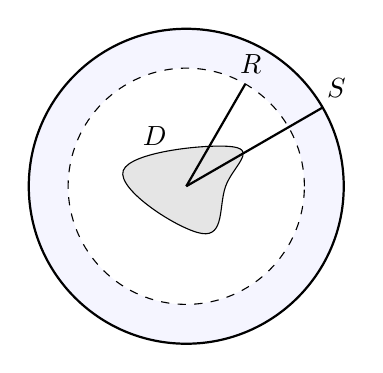
\begin{tikzpicture}
\fill [blue!4,even odd rule] (0,0) circle[radius=2cm] circle[radius=1.5cm];
\draw [dashed] (0,0) circle[radius=1.5 cm];
\draw [thick] (0,0) circle[radius=2 cm];
\draw[color=black] (-0.4,0.64) node {$D$};   
\draw[fill=gray!20] plot[smooth cycle,tension=.8]
 coordinates{(-0.8,0.2) (0.6,0.5) (0.5,0) (0.2,-.6)};  
\draw [thick] (0,0) -- (30:2cm) node[anchor=235] {$S$};
\draw [thick] (0,0) -- (60:1.5cm) node[anchor=255] {$R$};
\end{tikzpicture}
\caption{A null infinity layer with a scatterer. The outer boundary at $\rho=S$ corresponds to null infinity. The layer matches to the interior computation at the interface $\rho=R=r$.}
\label{fig:annulus}
\end{figure}

In the time domain, the hyperboloidal layer \cite{ZENGINOGLU20112286} implements this idea. In the frequency domain, we refer to it as a null infinity layer because one can use hyperboloidal and characteristic coordinates by choosing the height function $h$ accordingly. The main feature of the layer is that its outer boundary is at null infinity. 

A null infinity layer solves the Helmholtz equation for a rescaled variable in different coordinates. The solution at the outer boundary of the layer corresponds to the solution at infinity and is therefore of particular interest, especially for radiative problems. We can recover the global solution on the entire unbounded domain by reversing the transformations. 

Consider the setup in Fig.~\ref{fig:annulus}. We have a scatterer with boundary $D$. We use standard coordinates in the domain that extends from the scatterer to $r=R$. The boundary of the numerical domain is at $\rho=S$ and the null infinity layer has thickness $S-R$, shaded in light blue. The spatial coordinate mapping in the null infinity layer reads
\begin{align}\label{eq:layer}
g(\rho)=R+ \frac{\rho-R}{\Omega(\rho)} \quad \mathrm{where} \quad \Omega(\rho) = 1 - \frac{(\rho-R)^n}{(S-R)^n}\Theta(\rho-R)\,,
\end{align}
where $\Theta$ is the Heaviside step function and $n$ is an integer power. The height function remains as in \eqref{eq:h} with $K=1$. These choices guarantee a matched interface satisfying
\[ g(R) = R, \quad d_\rho g(R) = 1, \quad d_\rho^n g(R) = 0 \ \mathrm{for} \ n>1. \] 
The optimal choice of the coordinate transformation in the null infinity layer will depend on the problem. For example, \cite{bernuzzi2011binary} uses $n=4$ in the definition of $\Omega$ to get higher derivatives at the layer interface, and \cite{hilditch2018evolution} chooses a smooth transition function instead of the Heaviside function.


\subsection{Specific choices of free functions}
There is considerable freedom in the mapping $g(\rho)$ and the height function $h(\rho)$. A numerical analysis of the various choices is outstanding. The optimal choice will depend on the problem, but generally, the regularity of the transformed Helmholtz equation \eqref{eq:hyp_general} follows if $1-H^2\sim G\sim g^{-2}$ near the outer boundary at $\rho=S$. 

The simple example presented in Sect.~\ref{sec:simple} includes the following choices
\[ d=1, \quad F(\rho)=0, \quad g(\rho)=\tan \rho, \quad G(\rho) = \cos^2\rho, \quad h(\rho) =\tan\rho - \rho, \quad H(\rho)= \sin^2\rho\,.\]
The outer boundary is at $S=\tfrac{\pi}{2}$. We have $(1-H^2)/G = 1+\sin^2\rho$, and $G g^2 = \sin\rho$, so the transformed equation \eqref{eq:transformed} is regular at the outer boundary. 

For most numerical experiments presented in this paper, we specify the mapping $g$ and the height function $h$ as follows
\begin{align} 
\label{eq:g}
g(\rho) = \frac{\rho}{1-\rho} \quad &\mathrm{with}\quad G(\rho) \equiv \left(\frac{d g(\rho)}{d\rho}\right)^{-1} = (1-\rho)^2\,, \\
\label{eq:h}
h(\rho) = g(\rho) - \frac{\rho}{K} \quad &\mathrm{with}\quad H(\rho) \equiv G(\rho) \frac{d h(\rho)}{d\rho} = 1 - \frac{\Omega(\rho)}{K} 
\end{align}
where $K>0$ is a parameter that will be used to adapt the transformation to high-frequency wave propagation, and we define $\Omega(\rho):=\sqrt{G(\rho)} = 1-\rho$. 
The resulting Helmholtz equation reads
\begin{align}\label{eq:hyp_specific}
	\Omega^2 \partial_\rho^2 u & - 2\left(\Omega - \iu k \left(1-\frac{\Omega^2}{K}\right)\right) \partial_\rho u + \frac{1}{\rho^2}\triangle_{S^{d-1}} u + \nonumber \\
	             & \left[k^2 \left( \frac{2}{K} - \frac{\Omega^2}{K^2} \right) - \frac{(1-d)(3-d)}{4 \rho^2} + 2 \iu k \frac{\Omega}{K} \right] u = \frac{F}{\Omega^2} \left(\frac{\rho}{\Omega}\right)^{\tfrac{d-1}{2}} e^{-\iu k h}
\end{align}
The equation is regular at infinity where $G=0$ if the source term $F$ falls off sufficiently fast towards infinity. The transformed Helmholtz operator is essentially the Helmholtz operator in hyperbolic space \cite{stoll2016harmonic}. 


\subsection{Relationship to PML and PAL}
The most commonly used absorbing layer in the literature is the perfectly matched layer (PML) \cite{BERENGER1994185}. PML is equivalent to a complex coordinate transformation \cite{chew19943d}. It is very flexible and convenient to use in various coordinates \cite{collino1998perfectly}. Recently, an improved version has been proposed using a complex mapping and rescaling called the perfect absorbing layer (PAL) \cite{wang2017perfect, yang2021truly}. Both PML and PAL damp outgoing waves propagating through the layer.

To contrast these methods with the proposed null infinity layer, we demonstrate the transformations on the example of a one-dimensional, monochromatic, outgoing, plane wave $U(x)=e^{\iu kx}$. We present the calculations for the layer with $x>R$ to avoid carrying Heaviside functions through the expressions. A simple choice of PML reads 
\be\label{eq:pml} x(r) = r + \iu \sigma (r-R), \ee
where $\sigma$ is a free parameter. The PML plane wave solution becomes
\[ U_{\mathrm{PML}}(r) = U(x(r)) = e^{\iu k r} e^{- k \sigma (r-R)}. \]
The wave solution is damped exponentially in the layer where $r>R$. The damping is stronger for thicker layers and larger $\sigma$.

PAL applies a compactification to the complex coordinate transformation of PML (see (3.24) and (3.25) in \cite{yang2021truly}). The mapping is the same as \eqref{eq:layer} with $n=1$ up to a parameter which we set to one 
\[ r(\rho) = R + T(\rho), \quad \mathrm{with} \quad T(\rho) = \frac{(S-R)(\rho-R)}{S-\rho} = \frac{\rho-R}{\Omega(\rho)}\,. \]
The compression mapping leads to singular equations as we discussed in Sec.~\ref{sec:simple}. To remove the infinite oscillations at the domain boundary, PAL introduces a similar rescaling as the null infinity layer
\[ U_{\mathrm{PAL}}(\rho) = e^{-\iu k T(\rho)} U_{\mathrm{PML}}(r(\rho)) = e^{\iu k R} e^{-k \sigma T(\rho)}. \]
The PAL solution is infinitely damped near the outer boundary of the layer irrespective of the thickness, which gives improved decay estimates for the PAL solution than for the PML solution. This property is desirable for constructing a perfect absorbing layer, but it obstructs the recovery of the solution in the exterior domain. We do not need to artificially dampen the outgoing solution when we use a real compactification with the rescaling. The essential benefit of this approach is that the radiative solution becomes directly available at the outer boundary. We can construct the null infinity solution in the layer to take the same form as the solution in standard coordinates using $x=g(\rho)$ and $h(\rho) = g(\rho) - \rho$
\[ u_{\mathrm{NIL}}(\rho) = e^{-\iu k h(\rho)} U(x(\rho)) = e^{-\iu k (g(\rho)-\rho)} e^{\iu k g(\rho)} = e^{\iu k \rho}. \]
We can also recover the PAL solution without the damping by using a slightly different choice for the height function,  $h(\rho) = g(\rho) + R$.  

While the NIL solution looks the same as the standard plane-wave solution, the transformed Helmholtz equation looks different from the Helmholtz equation in standard coordinates. In particular, the transformed equation is regular throughout the domain in compressed coordinates and does not require boundary data. 

%%%%%%%%%%%%%%%%%%%%%%%%%%%%%%
\section{Numerical experiments}\label{sec:numerical}
%%%%%%%%%%%%%%%%%%%%%%%%%%%%%%

\subsection{Experiment 1: Plane wave in 1D}\label{sec:oned}
One-dimensional examples are generally not representative of the difficulties related to the outer boundary problem. In our case, however, the essential elements of null infinity compactification are present in one dimension because the transformation acts in the radial direction. Once radial and angular directions are separated, the technique in higher dimensions is similar to its implementation in one dimension because the dynamics of outgoing waves in the asymptotic region is essentially one-dimensional.

Consider the following one-dimensional problem on an unbounded domain
\begin{equation}
	\label{eq:oneD}
	\begin{gathered}
		U_{xx} + k^2 U = 0, \quad \mathrm{in} \ x\in[a,\infty),\\
		U|_{x=a} = \Psi,\\
		\lim_{x\to\infty} (U_x - \iu k U) = 0,
	\end{gathered}
\end{equation}
A simple solution to the above system is the plane wave, $U=e^{\iu k x}$, obtained with the Dirichlet boundary condition $\Psi=e^{\iu k a}$. 

Setting $d=1$ in \eqref{eq:hyp_specific} with vanishing source, we get the transformed problem
\begin{equation}
	\label{eq:hyp_1d}
	\begin{gathered}
		\Omega^2 u_{\rho\rho} - 2 \left(\Omega-\iu k \left(1-\frac{\Omega^2}{K}\right) \right) u_\rho + \left[k^2 \left(\frac{2}{K}-\frac{\Omega^2}{K^2}\right) + 2 \iu k \frac{\Omega}{K} \right] u = 0,\\
		u|_{\rho=\rho_a} = e^{-\iu k (a-\rho_a/K)}\Psi,
	\end{gathered}
\end{equation}
where $\rho_a=\tfrac{a}{1+a}$ and $\Omega(\rho)=1-\rho$. We do not impose the Sommerfeld condition separately because it follows from evaluating the equation at infinity 
\[ u_\rho - \iu \frac{k}{K} u = 0,   \quad \mathrm{at} \ \rho=1. \]
The wavenumber of an outgoing plane wave with null infinity compactification is divided by $K$. The solution reads $u(\rho)=e^{\iu \tfrac{k}{K} \rho}$. We will exploit this modification to compute solutions with high wave numbers.

We plot the real parts of the original solution, $U(x)$, and the transformed solution, $u(\rho)=e^{-ikh(\rho)}U(\rho)$ in Fig.~\ref{fig:oned} with $a=1$ and $k=40$. We restrict the plot in $x$ to $x\in[1,2]$. The domain in $\rho$ includes the point at infinity: $\rho\in[\tfrac{1}{2},1]$.
\begin{figure}[tbhp]
	\centering
	\includegraphics[scale=0.4]{figs/st_oned}
	\includegraphics[scale=0.4]{figs/hyp_oned.pdf}
	\caption{Real parts of the plane wave solution and its transformation in one dimension for $k=40$. The transformed solution is plotted on the right panel for $K=1$ and $K=k$. The domain of the mapped solution corresponds to an infinite domain, and the flattening of the oscillations is controlled by the parameter $K$.}
	\label{fig:oned}
\end{figure}

The plane wave solution has more oscillations across the plotted domain than the hyperboloidal solution, even though the hyperboloidal solution extends to infinity. The freedom in the transformation can be exploited to flatten the oscillations even further, as demonstrated by the solid curve on the right panel of Fig.~\ref{fig:oned}, which corresponds to the transformed solution with $K=k$.

We solve \eqref{eq:oneD} and \eqref{eq:hyp_1d} using two numerical discretizations: a finite difference scheme of second-order and a spectral-collocation scheme based on Chebyshev polynomials. For solving \eqref{eq:oneD}, the outer boundary data is taken from the exact solution. For solving \eqref{eq:hyp_1d}, the finite difference scheme uses one-sided difference operators at the outer boundary with no boundary data imposed. The spectral-collocation scheme does not require an outer boundary treatment because the principal part is degenerate at infinity which implies a behavioral condition in the terminology of Boyd \cite{boyd2001chebyshev}.

\begin{figure}[tbhp]
	\centering
	\includegraphics[scale=0.4]{figs/fd_err_1d}
	\includegraphics[scale=0.4]{figs/sp_err_1d}
	\caption{Errors for second order finite difference (left) and Chebyshev spectral (right) solvers in one dimension for $k=40$ for the solution of the 1D problem \eqref{eq:hyp_1d}.}
	\label{fig:errs_oned}
\end{figure}

Figure \ref{fig:errs_oned} shows the corresponding numerical errors for the two schemes. The spectral method is more accurate, as expected. The plots also demonstrate the increased efficiency of the transformed solution for $K=k$. In this particular example, one can freely choose a large $K$. In fact, the characteristic foliation with $h(\rho) =g(\rho)$ leads to the transformed solution $u(\rho)=1$. 

\subsubsection{Experiment 2: Single mode in 2D} 
We consider the source free Helmholtz equation in 2D. We set $d=2$ and $F=0$ in \eqref{eq:helm_sph} and write the equation as a sequence of 1-D equations by expanding the unknown in polar coordinates, $U=\sum U_m(r) e^{\iu m \theta}$. Dropping the subscript $m$, we write
\begin{equation}
	 U_{rr} + U_r + \left(k^2 - \frac{m^2}{r^2}\right)U = 0.
\end{equation}
Applying null infinity compactification using \eqref{eq:g} and \eqref{eq:h} gives 
\begin{equation}
\label{eq:hyp_2d}
	\Omega^2 u_{\rho\rho} - 2 \left(\Omega-\iu k \left(1-\frac{\Omega^2}{K}\right) \right) u_\rho + \left[k^2 \left(\frac{2}{K}-\frac{\Omega^2}{K^2}\right) - \frac{m^2-\tfrac{1}{4}}{\rho^2}  + 2 \iu k \frac{\Omega}{K} \right] u = 0,\\
\end{equation}
Solutions satisfy at the outer boundary the relationship
\[ u_\rho - \iu \left(\frac{k}{K} - \frac{m^2-\tfrac{1}{4}}{2k}\right)u = 0.  \]
This expression suggests that increasing $K$ may not be as effective as in the one dimensional example, especially for large mode numbers. Nevertheless, for high-frequency wave propagation with large $k$, modifying $K$ accordingly should lead to a more efficient solver.

A single mode solution in 2D is given through Hankel functions of the first kind as  $U(r, \theta) = H_m^{(1)}(k r) e^{\iu m \theta}$. After angular decomposition, we get the following expressions for the radial solution in standard and transformed coordinates
\begin{equation}\label{eq:hankel_soln}
	U(r) = H_m^{(1)}(k r), \qquad u(\rho) = \sqrt{r(\rho)} e^{\iu \tfrac{k}{K} \rho} \, \bar{H}_m^{(1)}\left(k r(\rho)\right),
\end{equation}
where $r(\rho)=\rho/\Omega$ and $\bar{H}_{m}^{(1)}$ denotes the exponentially scaled Hankel function defined as $\bar{H}_{m}^{(1)}(z) := e^{-\iu z} H_{m}^{(1)}(z)$. Improved numerical behavior of exponentially scaled Bessel functions for large argument are exploited in many software libraries \cite{amos1986algorithm, 2020SciPy-NMeth}. We can view this exponential scaling geometrically as evaluation along characteristic hypersurfaces of the underlying Minkowski spacetime in line with the time transformation described in step (ii) and the discussion in Sec.~\ref{sec:time} (see also \cite{ZengFramework}).

Many engineering applications require the computation of the far-field pattern. The far-field solution at infinity can be obtained from the asymptotic behavior of the scaled Hankel function. For large $z$, we have \cite{olver1972bessel}
\[ \bar{H}_{m}^{(1)}(z) = \sqrt{\frac{2}{\pi z}} e^{-\iu \pi \left(\tfrac{m}{2}+\tfrac{1}{4} \right)} + O\left(\frac{1}{z^{3/2}}\right) \]
The transformed solution \eqref{eq:hankel_soln} evaluated at null infinity reads
\[ u(1) = \sqrt{\frac{2}{\pi k}} e^{\iu \left(\tfrac{k}{K}- \pi \left(\tfrac{m}{2}+\tfrac{1}{4} \right) \right)}\,. \]
The far-field pattern is directly accessible at the outer boundary of the domain.

The radial dependence of the transformed solution is plotted for $k=40$ and $m=20$ in Fig.~\ref{fig:twod}. We observe a similar flattening of the oscillations across the domain as in the 1D case. The choice $K=k$ does not remove the oscillations as much as in the 1D case because of the impact of the mode number $m$. The numerical error for the spectral-collocation method is plotted on the right panel of Fig.~\ref{fig:twod}. 


\begin{figure}[tbhp]
	\centering
	\includegraphics[scale=0.4]{figs/hyp_twod}
	\includegraphics[scale=0.4]{figs/sp_err_2d}
	\caption{Left panel: Null infinity compactification of the single mode Hankel function for $k=40$ and $m=20$. Due to the mode number $m$, the choice $K=k$ does not remove the oscillations as much as in the 1D case (compare Fig.~\ref{fig:oned}). Right panel: Numerical error comparison between the standard method with exact boundary conditions and the hyperboloidal method with two choices for $K$. The efficiency gain from setting $k=K$ is not as large as in 1D (compare Fig.~\ref{fig:errs_oned}). }
	\label{fig:twod}
\end{figure}



\subsubsection{Experiment 3: Scattering of incoming waves}
This section discusses a scattering problem both in NIC and NIL coordinates. In NIC, the transformation is applied throughout the entire numerical domain, while in NIL, it is restricted to a thin outer layer.  It may be beneficial in certain applications to use NIL, but the layer should be generally avoided if the waves are predominantly outgoing. For the calculations, we set the height function as in \eqref{eq:h} with $K=1$,  and the spatial transformation as in \eqref{eq:g} for NIC and \eqref{eq:layer} for NIL. The equation is given in \eqref{eq:hyp_2d} where we set $K=1$.

We consider a plane wave in the $x$-direction, $e^{\iu k x} = e^{\iu k r \cos\theta}$, scattered off a circle of radius $R_0=1$. The incident plane wave does not satisfy the Sommerfeld radiation condition in 2D and therefore is not regular at null infinity. The scattered solution is outgoing at infinity and is therefore regular. The total field is the sum of the impinging field and the scattered field, implying the following Dirichlet boundary condition for the scattered field:
\begin{equation}\label{eq:dirichlet}
	U(r,\theta)|_{r=R_0} = - e^{\iu k R_0 \cos\theta}.
\end{equation}
We write the solution satisfying the Sommerfeld radiation condition as a series expansion (as in, for example, \cite{britt2010compact, yang2021truly})
\[ U(r,\theta) =  \sum_{|m|=0}^{\infty} c_m H_{m}^{(1)}(k r) e^{\iu m \theta} \,, \]
where the coefficients, $c_m$, are determined from a Fourier expansion by requiring that the Dirichlet condition \eqref{eq:dirichlet} is satisfied at the scattering surface:
\[ c_m = \frac{1}{H_{m}^{(1)}(k R_0)} \frac{1}{2\pi} \int_{-\pi}^{\pi} -e^{\iu k R_0 \cos\theta} e^{-\iu m \theta} d\theta = 
- \frac{\iu^m J_m(k R_0)}{H_{j}^{(1)}(k R_0)}. \]
The $J_m$ are Bessel functions. We obtain the transformed boundary data and solution by scaling-out the oscillatory decay and compactifying as in \eqref{eq:hankel_soln}. The boundary data reads
\[ u(\rho_0,\theta)= \sqrt{R_0} e^{-\iu k (R_0-\rho_0)} U(R_0,\theta) %= - \sqrt{R_0} e^{\iu k R_0 \left(\cos\theta-\tfrac{R_0}{1+R_0}\right)}\,.
\]
The transformed solution reads
\begin{equation}\label{eq:soft_soln}
	u(\rho,\theta) = \sqrt{r(\rho)} e^{\iu k\rho} \sum_{|m|=0}^{\infty} c_m \bar{H}_{m}^{(1)}\left(k r(\rho)\right) e^{\iu m \theta},
\end{equation}
Three representations of the solution in (a) standard, (b) NIC, and (c) NIL coordinates are plotted in Fig.~\ref{fig:soft_sound}. The black interior circle on panel (c) marks the interface at $\rho=R$. The solution for $\rho<R$ agrees identically with the standard representation on panel (a). 

\begin{figure}[ht]
  \subfloat[Standard coordinates.]{
	\begin{minipage}[c][1\width]{
	   0.32\textwidth}
	   \centering
	\includegraphics[width=\textwidth]{figs/soft_sound_standard.png}
	\end{minipage}}
 \hfill 	
  \subfloat[NIC coordinates.]{
	\begin{minipage}[c][1\width]{
	   0.32\textwidth}
	   \centering
	   \includegraphics[width=\textwidth]{figs/soft_sound_hypal.png}
	\end{minipage}}
 \hfill	
  \subfloat[NIL coordinates.]{
	\begin{minipage}[c][1\width]{
	   0.32\textwidth}
	   \centering
	   \includegraphics[width=\textwidth]{figs/soft_sound_nil.png}
	\end{minipage}}
\caption{Scattering of an incident wave for $k=40$ in (a) standard coordinates on $r\in[1,2]$; (b) NIC coordinates on $\rho\in[0.5,1]$; and (c) NIL coordinates on $\rho\in[1,2.2]$. The black circle on the NIL solution on panel (c) depicts the interface at $R=2$. The solution for $\rho<R$ matches identically the solution depicted on panel (a). The harmonic content of the NIC representation on (b) is smaller than the NIL representation on (c), which leads to a more efficient computation.}
\label{fig:soft_sound}
\end{figure}



The NIC representation shows fewer waves along the radial directions in accordance with the flattening property of hyperboloidal compactification. The NIL representation distorts the waves in the layer transporting them to null infinity. It also has a higher harmonic content than the NIC representation. Therefore, this particular problem should use the NIC representation. We present in Fig.~\ref{fig:twod_scattering} convergence results for solving the Helmholtz equation in NIC representation both with spectral (left panel) and 2nd order finite difference (right panel) methods. Spectral methods are superior in such problems.

\begin{figure}[tbhp]
	\centering
	\includegraphics[scale=0.41]{figs/spectral_2d.png}
	\includegraphics[scale=0.41]{figs/fd_2d.png}
	\caption{Convergence for the solution of the scattering of an incident plane wave with $k=40$ using spectral (left) and 2nd order finite difference (right) methods. }
	\label{fig:twod_scattering}
\end{figure}

\section{Summary and Discussion}
% Advantages
The main idea of this paper is the following directive: Scale out the oscillatory decay and compactify \eqref{eq:summary}. Applying this simple directive leads to equation \eqref{eq:hyp_general} which has various advantages for scientific computation. First, the equation does not require formulating an artificial outer boundary problem. One solves the degenerate equation without imposing boundary data because the equation geometrically incorporates the no-incoming radiation condition through a behavioral boundary. This property of the equation also simplifies its discretization. For example, among the motivations for constructing compact finite difference operators with narrow stencils is the boundary treatment \cite{britt2010compact}. In contrast, null infinity compactification allows us to apply high-order finite-difference operators using one-sided stencils near the outer boundary. In spectral methods, the function space automatically incorporates the behavior near the boundary.

There was much discussion about time and characteristic speeds in this paper. It is unusual to discuss time and characteristic speeds in a paper on the Helmholtz equation. After all, there is no time in the equation. However, the Helmholtz equation is deeply connected to the wave equation through the time-harmonic ansatz. The unification of space and time into spacetime by Minkowski suggests that we can treat time just like another coordinate. The compactification procedure needs to take time into account (Penrose).

Another advantage of null infinity compactification is access to the asymptotic solution. In many scientific and engineering applications, we need to measure the outgoing radiation, such as the echo area in acoustics, the radar cross-section in electromagnetics, or the gravitational waveform in general relativity. Truncating the problem domain makes the extraction of such quantities cumbersome. With null infinity compactification, we can read off the radiation from the numerical solution performed on a relatively small domain directly without post-processing. %A potential direction for research would be applying this method to a real-world problem in engineering, such as the computation of the radar cross-section of an airplane using high-order finite element methods solving Maxwell's equations. 

The flexibility of the method allows us to adapt the coordinates to the problem. For example, black hole perturbations propagate both to infinity and the black hole. We can adjust the height function to incorporate this behavior into the equation resulting in behavioral boundaries at both ends of the domain (black hole horizon and null infinity)\cite{ZengFramework}. Similarly, suppose the geometry of a wave scattering problem has preferred directions of wave propagation. In that case, one can incorporate these into the height function to improve the efficiency of the numerical method.

% Future directions and limitations

The relationship of rescalings with time transformations puts existing literature on Helmholtz equations into a geometric framework. We understand the exponential rescaling in PAL and infinite elements as transformations to a characteristic coordinate system. The rescaling of the asymptotic decay corresponds to the conformal compactification of the underlying spacetime. This unified framework allows us to extend existing methods to general height functions to incorporate variable propagation speeds and heterogeneous media.
 
Currently, the method is limited to smooth outer boundaries. This restriction comes from the topology of null infinity: cross-sections of future null infinity have spherical topology \cite{Penrose65, Geroch}. We can use ellipsoidal or prolate spheroidal coordinates to simulate scattering from long objects. More generally, we can parametrize a smooth boundary as demonstrated in \cite{yang2021truly}. However, as presented in this paper, null infinity compactification is not readily applicable to Cartesian or polygonal domains.

The method should be further investigated in real-world applications where restriction of the transformations to a layer may be necessary. Another avenue of research is the numerical analysis of the transformed equation \eqref{eq:hyp_general} for suitable choices of height function and compactification. The nature of the transformations and the outcomes of numerical experiments suggest that null infinity compactification is local, exact, and stable. A detailed numerical analysis of these properties is lacking. Such research would also be helpful to obtain guidelines for choices of free functions and parameters involved in the transformations, such as the thickness of the null infinity layer or the shape of the height function.

%%%%%%%%%%%%%%%%%%%%%%%%%%%%%%
%%%%%%%%%%%%%%%%%%%%%%%%%%%%%%
\appendix
%%%%%%%%%%%%%%%%%%%%%%%%%%%%%%
%%%%%%%%%%%%%%%%%%%%%%%%%%%%%%

%%%%%%%%%%%%%%%%%%%%%%%%%%%%%%
\section{Null infinity and Penrose diagrams}
\label{sec:app_penrose}
%%%%%%%%%%%%%%%%%%%%%%%%%%%%%%
The method presented in this paper relies on relativistic techniques. Studies on compactification in the applied mathematics literature only consider compactification in space \cite{GroschOrszag77, boyd1982optimization, shen2009some}. For wave propagation problems, however, the time direction must be considered as well. 

Penrose presented compactification of spacetime in a series of papers starting in 1963 \cite{Penrose, Penrose65}. In this appendix, we collect the main ideas as a starting point for the interested reader. 

Spacetime distances are measured by the Minkowski metric. The metric takes the following form in spherical coordinates $\{t,r,\theta,\varphi\}$
\[ \eta  = -dt^2 + dr^2  + r^2 d\sigma^2, \]
where $d\sigma^2 = d\theta^2 + \sin^2\theta d\varphi^2$, the standard metric on the unit sphere. The wave operator is the d'Alembert operator for this metric
\[ \Box = \eta^{\mu\nu} \partial_\mu \partial_\nu =  \]


%%%%%%%%%%%%%%%%%%%%%%%%%%%%%%
\section{Numerical methods}
%%%%%%%%%%%%%%%%%%%%%%%%%%%%%%
We briefly present the numerical methods used in the experiments of Sect.~\ref{sec:numerical}. We demonstrate the discretization in one representative dimension denoted by $x$. The implementation is publicly available at the compendium site for the paper \cite{compendium}.

%%%%%%%%%%%%%%%%%%%%%%%%%%%%%%
\subsection{Finite Difference Method}
Finite differences are the easiest option to approximate derivatives. We discretize the solution domain with a uniform grid spacing. Let $N$ be the number of grid cells and set $x_i=i h$ with the grid spacing $h=1/N$. A function $u(x)$ has values on the grid denoted by $u_i=u(x_i)$. We approximate derivatives by matrix multiplication as follows
\[ d_x u|_{x=x_i} \approx \sum_j {D_{ij}^{(1,o)}} u_j, \qquad d_x^2 u|_{x=x_i} \approx \sum_j D_{ij}^{(2,o)} u_j, \]
where $o$ denotes the order of accuracy. The coefficients form a sparse matrices.

\subsubsection{Interior stencils}
We give the spatial differentiation matrices through their action on a grid vector. 
Second order spatial differentiation matrices 
\[ \sum_j {D_{ij}^{(1,2)}} u_j  = \frac{1}{2h} (u_{i+1}- u_{i-1}), \quad \sum_j {D_{ij}^{(2,2)}} u_j = \frac{1}{h^2} (u_{i+1}- 2 u_i + u_{i-1}). \]
Fourth order order operators are 
\[ \sum_j {D_{ij}^{(1,4)}} u_j  = \frac{1}{2h} (u_{i+1}- u_{i-1}), \quad \sum_j {D_{ij}^{(2,4)}} u_j = \frac{1}{h^2} (u_{i+1}- 2 u_i + u_{i-1}). \]

Higher-order derivatives have wider stencils. The matrices are implemented up to 6th order as sparse matrices using the Python package scipy \cite{2020SciPy-NMeth}.


\subsubsection{Boundary Treatment}
One-sided differencing is used at the endpoints. 

One-sided differencing at the right boundary, $x_N$, gives
\[ \sum_j {D_{Nj}^{(1,2)}} u_j = \frac{1}{2h}(u_N - 4 u_{N-1} + 3 u_{N-2}),\]
and
\[ \sum_j {D_{Nj}^{(2,2)}} u_j = \frac{1}{h^2}(2 u_N - 5 u_{N-1} + 4 u_{N-2} - u_{N-3}).\]

We impose Dirichlet boundary conditions in the inner boundary. 
Second order boundary:
\[ -\frac{a}{h^2} + \frac{b}{2h} \]
Fourth order boundary:
\[ -\frac{-10a}{12 h^2} + \frac{3 b}{12h} \]
Sixth order boundary:
\[ -\frac{a}{h^2} + \frac{b}{2h} \]

%%%%%%%%%%%%%%%%%%%%%%%%%%%%%%
\subsection{Chebyshev Collocation Method}


%%%%%%%%%%%%%%%%%%%%%%%%%%%%%%
\subsection{Weighted spectral-Galerkin Method}


\section*{Acknowledgments}
I thank the Institute for Physical Science and Technology and its director Konstantina Trivisa for providing me space and time to perform this research. I thank Rodrigo Panosso Macedo, Ricardo Nochetto, and Eitan Tadmor for valuable discussions, and Jie Shen for reminding me of the references \cite{wang2017perfect, yang2021truly}. 


\bibliographystyle{siam}
%\bibliographystyle{siamplain}

\bibliography{refs}

\end{document}
